% \textbf{Notation.}
Let $\mathcal{G} = (\mathcal{V}, \mathcal{E}, \mathbf{X})$ be an undirected graph, with $\mathcal{V}$ the set of nodes and $\mathcal{E} $ the set of edges. We denote by $N = |\mathcal{V}| $  the number of nodes of   $\mathcal{G}$.  
$\mathcal{N}_u$ is the neighborhood of the node $u$, and $d_u = |\mathcal{N}_u|$ is its degree.
%Thus, if node $i$ is adjacent to nodes $j$, and $k$, we write $\Gamma(i) = \{j, k\}$, and $|\Gamma(i)| = 2$.
$\mathbf{D}$ $\in \mathbb{R}^{N \times N}$ is the degree matrix, a diagonal with  entries 
$D_{u u} = d_u$. Each node $u$ has feature vector
$\mathbf{x}_u \in \mathbb{R}^m$. The  feature
matrix  $\mathbf{X} \in \mathbb{R}^{N \times m} $ stacks all the feature vectors. $\mathbf{A} \in \{0, 1\}^{N \times N}$ is the graph's adjacency matrix, with $A_{uv} = 1$ if $(u, v) \in \mathcal{E}$  and $A_{uv} = 0$ otherwise.

\textbf{Graph Neural Networks for Graph Classification. }In graph classification, each sample in the dataset, $\mathcal{D}$, is a graph, i.e.,  $\mathcal{D} = \{\mathcal{G}^{i}, \mathbf{y}_i\}_{i = 1}^{n}$, where $\mathcal{G}^{i} = (\mathcal{V}^i, \mathcal{E}^i, \mathbf{X}^i)$, and $\mathbf{y}_i \in \{0, 1\}^{|C|}$ is its class associated one-hot encoded representation.
%that attach to $\mathcal{G}^i$, one among $|C|$ possible labels. 
We represent the set of labels for $\mathcal{D}$ as $\mathbf{y} \in \{0, 1\}^{n \times |C|}$. More simply we use $c_i$ to express the class of sample $i$. $\mathbf{X}^i \in \mathbb{R}^{N_i \times m}$, and $\mathbf{A}^i \in \mathbb{R}^{N_i \times N_i}$ are the feature and adjacency matrices of graph $i$ respectively.
% In the case of learning under label noise, $c_i$ may differ from the ground truth, except for the labels in the test set.  In this context, GNNs are utilized to extract features from graph-structured data. According to the message passing formalism \cite{messagepassing}, each feature matrix in $\mathbf{X}^i \hspace{0.1cm} \forall i \in \{1, ..., n\}$ gets updated within the GNN, retrieving a new set of latent features $\mathbf{Z}^i \in \mathbb{R}^{N_i \times m'}$ of the graph $\mathcal{G}^i$. Along the forward pass, we denote the intermediate representations as $\mathbf{H}_i^l, 0 \leq l \leq L$, for each layer in the GNN, up to the $L$-$th$ one. In particular, we may express $\mathbf{X}^i \equiv \mathbf{H}^0_i$, and $\mathbf{Z}^i \equiv \mathbf{H}^L_i$. Provided a set of weights $\mathbf{W}_l$, and $\mathbf{\Omega}_l$ for the layer $l$, we can write, similarly to \cite{messagepassing}, the message-passing update rule for a graph $i$ as follows.
% $ \mathbf{H}^{l+1}_i = UP_{\mathbf{\Omega}_l}(\mathbf{H}^{l}_i, AGGR_{\mathbf{W}_l}(\mathbf{H}^{l}_i, \mathbf{A}^i)) \;  0 \leq l \leq L \text{ \hspace{0.25cm}} l \in \mathbb{N},$
% having $UP_{\mathbf{\Omega}_l}$, and $AGGR_{\mathbf{W}_l}$ as the \textit{update} and \textit{aggregation} function of the message-passing.
In the case of learning under label noise, in the training data $c_i$ may differ from the ground truth. In this setting, GNNs are employed to extract features from graph structured data. In the message passing formalism~\citet{messagepassing}, each feature matrix $\mathbf{X}^i \hspace{0.1cm} \forall i \in \{1, ..., n\}$ is iteratively updated within the GNN, yielding a new set of latent features $\mathbf{Z}^i \in \mathbb{R}^{N_i \times m'}$ for the graph $\mathcal{G}^i$. We denote the intermediate representations as $\mathbf{H}_i^l,\; 0 \leq l \leq L$, for each GNN layer up to the $L$-th one. We identify $\mathbf{X}^i \equiv \mathbf{H}^0_i$ and $\mathbf{Z}^i \equiv \mathbf{H}^L_i$. Given a set of weights $\mathbf{W}_l$ and $\mathbf{\Omega}_l$ for layer $l$, the message-passing update rule for graph $i$ is:
\begin{equation}
\mathbf{H}^{l+1}_i = UP_{\mathbf{\Omega}_l}\left(\mathbf{H}^{l}_i,\; AGGR_{\mathbf{W}_l}\left(\mathbf{H}^{l}_i,\; \mathbf{A}^i\right)\right), \quad 0 \leq l \leq L,\; l \in \mathbb{N},
\end{equation}
where $UP_{\mathbf{\Omega}_l}$ and $AGGR_{\mathbf{W}_l}$ denote the \textit{update} and \textit{aggregation} functions of the message passing mechanism.
% Next, node representations are aggregated into a final graph representation using a learnable, permutation-invariant readout function $f_{\theta}: \mathbb{R}^{m'} \rightarrow \mathbb{R}^{|C|}$, which could be a sum, mean, or graph pooling method \cite{diffpool}. The output, $ \mathbf{\hat{y}}_i$, is the one-hot encoded class prediction.
% Next, node representations \( \mathbf{Z}^i \in \mathbb{R}^{N \times m'} \) are  transformed into class probabilities using a learnable, permutation-invariant function \( f_{\theta}: \mathbb{R}^{N_i \times m'} \rightarrow \mathbb{R}^{|C|} \), Probabilities are then expressed as one-hot encoded \( \mathbf{\hat{y}}_i \).
After obtaining the final node representations \( \mathbf{Z}^i \in \mathbb{R}^{N_i \times m'} \), a learnable, permutation-invariant function \( f_{\theta}: \mathbb{R}^{N_i \times m'} \rightarrow \mathbb{R}^{|C|} \) is applied to transform them into class probabilities. The predicted output is then represented as a one hot encoded vector \( \mathbf{\hat{y}}_i \).


% Then, a readout function is utilized to
% summarize node representations in a final graph representation. 
%The new nodes' representations $\mathbf{Z}^i$ are then functional to a downstream task.
%typically node classification, graph classification, or link prediction. 
% This is done by applying a learnable readout function $f_{\theta}: \mathbb{R}^{m'} \rightarrow \mathbb{R}^{|C|}$ to the whole set of nodes' representation,
%as follows:
%\begin{equation}
%    \mathbf{\hat{y}}_i = f_{\theta}(\mathbf{Z}^i),
%\end{equation}
% $f_{\theta}$ is typically a permutation invariant function that returns the final prediction, it may be a sum, mean or a graph pooling method \cite{diffpool}. 
% We denote by $ \mathbf{\hat{y}}_i$ the one-hot encoded representation of the class predicted by the network.
%More specifically, $f_{\theta}$ computes the prediction in a one-hot encoded form ($\mathbf{\hat{y}_i \in \mathbb{R}^{|C|}}$), while we denote as $\mathbf{z}_i \in \mathbb{R}^{m''}$ the vector representation for graph $i$, that is computed before the final prediction but after the pooling operation i.e. after having aggregated the node features.\\

\textbf{Dirichlet Energy on graphs.} 
% The Dirichlet Energy  of a graph $E^{dir}$ measures how much the signal between adjacent nodes is smoothed and is defined as 
% \begin{equation}
% \label{eq: dirichlet}
%    E^{dir}(\mathbf{X}) := \frac{1}{2} \sum_{(u,v) \in \mathcal{E}} \| (\nabla \mathbf{X})_{uv} \|^2
% \end{equation}
% where $(\nabla \mathbf{X})_{uv} := \frac{\mathbf{x}_v}{\sqrt{d_{v}}} - \frac{\mathbf{x}_u}{\sqrt{d_{u}}}$ is the gradient of edge $(u,v)$, and $\|\cdot\|$ denotes the $l_2$ norm of a vector. Similar to physical systems, this energy is used to understand the underlying dynamics of the nodes' features. When $E^{dir}$ decreases we assume a smoothing behavior, otherwise a sharpening one.
We now define the Dirichlet energy for graph data: \( E^{dir} \), which quantifies the smoothness of a scalar or vector field defined over the nodes of a graph. For a graph \( \mathcal{G}^i = (\mathcal{V}^i, \mathcal{E}^i) \) with node representation matrix \( \mathbf{Z}^i \in \mathbb{R}^{N_i \times m'} \), where \( \mathbf{Z}^i \) denotes the latent features of nodes, the Dirichlet energy is defined as:
\begin{equation}
%E^{dir}(\mathbf{Z}^i) = \sum_{(u,v) \in \mathcal{E}^i} \left\| \frac{\mathbf{Z}^i_{u}}{d_u} - \frac{\mathbf{Z}^i_{v}}{d_v} \right\|_2^2  
E^{dir}(\mathbf{Z}^i) = \sum_{(u,v) \in \mathcal{E}^i} \left\| \mathbf{Z}^i_{u}/d_u - \mathbf{Z}^i_{v}/d_v \right\|_2^2
\label{eq:edir-edge}
\end{equation}
where \( \mathbf{Z}^i_{u}\) denotes the representation of node $u$. $E^{dir}(\mathbf{Z}^i)$ sums the squared differences of the feature vectors across all edges. Intuitively, \( E^{\text{dir}} \) is small when the connected nodes have similar representations (smooth signal), and large when the neighboring nodes differ (indicating sharpening).


%  \begin{figure}[htbp]
%   \centering
%         %\includegraphics[scale = 0.25]{Neurips/Screenshots/gin_drchi_6Classes_30/differntnoise_Dirchi_CE_NCOD.png}
%         %
\includegraphics[page=1,width=1.0\textwidth]{Neurips/figures/fig8b}
%         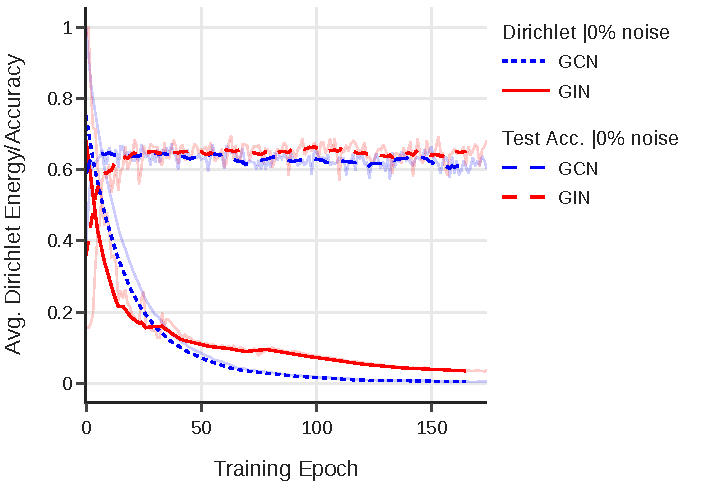
\includegraphics[width=.5\textwidth]{AISTATS/figures/gin_gcn_dir.pdf}
%         \caption{Comparison of average Dirichlet energy and Accuracy evolution on PPA dataset, using Cross-Entropy (CE) in both GIN and GCN models (Dirichlet Energy is normalized to scale for comparison).}
%         \label{fig:gin_gcn_dir}
% \end{figure}
 


% Notice that for the loss term $\mathcal{L}_3$ we have that the Kullback–Leibler (KL) divergence is computed between the following distribution, for a batch of graphs $B$ of size $|B|$ we obtain the prediction of the model for it: $f_{\theta}(B) \in \mathbb{R}^{|B| \times C}$. We then compute the diagonal of the matrix obtained by the product of the matrix $f_{\theta}(B) $ and the matrix $y_{B}$ having dimension $ C \times |B| $ that in each column contains the one hot encoded representations of the samples' labels. 
% $  \text{diag} (f_{\theta}(B) \cdot y_{B})  \in \mathbb{R}^{|B|} $ indeed $f_{\theta}(B) \cdot y_{B}$ has on the diagonal the probability output of the model for the real class.
% Notice that also $u_{B}$ is a vector of size $|B|$ containing the parameter $u$ for the vaious samples in the batch. 
% In the term $\mathcal{L}_3$ we compute the KL divergence between the distribution of $  \text{diag} (f_{\theta}(B) \cdot y_{B}) $ and the $u_{B}$.



%\begin{itemize}
%     \item For graph classification the representation of the graph will mostly rely on the lower frequencies because this is common to all nodes, meaning enhance them. This will lead to smoothing. 
% \end{itemize}
% \begin{theorem}
%     Let us assume we have a linear graph neural network 
%     $$ Y = W_2 ( F + AFW_1 )$$
%     If $W_2$ only has positive eigenvalues in the lower frequencies that means we will see that the features on the graph nodes $F$ will smooth. 
% \end{theorem}


% \begin{theorem}
%     Let us assume we have a linear graph neural network 
%     $$ W^2 ( F + AFW^1 )$$
%     I $W^2$ only has positive eigenvalues in the lower frequencies which means we will see that the features on the graph nodes $F$ will smooth. 
% \end{theorem}


% \section{Robustness to Label Noise in GNN-GC}

% Here we present the problem, we say that we show empirically that GNN-GC is often robust to label noise unless the dataset is small and graphs are sparse.